\section{Analysis of Datasets for Inference of Emotional Expressions}
\label{sec:datasets}

%In this chapter, we outline the methodology employed for the comparative analysis of the \affectnet{} and \emotic{} datasets.

% \subsection{Comparing Datasets}

% To assess the two datasets, we conducted a comparative analysis to identify similarities and dissimilarities in terms of:
% \begin{itemize}
% \item Annotation granularity and emotion categories
% \item Data distribution and imbalance
% \item Annotation reliability and consistency within and between the datasets
% \end{itemize}

% Through our comparative analysis, we aimed to identify key differences between the \affectnet{} and \emotic{} datasets, which may impact the performance and generalization capability of emotion recognition models trained on these datasets.



% ********************************
% ** Subsection about the dataset comparison **
% ********************************

\begin{figure}[t]
\centering
\hspace{-1cm}
\begin{subfigure}{0.6\linewidth}
  \includegraphics[width=\linewidth]{pictures/affectnet/example_image.pdf} 
    \caption{AffectNet-8 (\textit{anger})}
    \label{body}
    \end{subfigure} \hspace{-1cm}
\begin{subfigure}{0.6\linewidth}
    \includegraphics[width=\linewidth]{pictures/emotic/example_image.pdf}
        \caption{EMOTIC (\textit{disconnection})}
    \end{subfigure}
    \caption{Example images from AffectNet-8 and EMOTIC.}
    \label{fig:example-imgs}
\end{figure}


\begin{table}[t]
\centering
\begin{tabular}{ r | c | c }
\hline
 \textbf{Property} & \textbf{\affectnet{}-8} & \textbf{\emotic{}} \\ 
\hline
 Train Images & 287,651 & 23,266 \\
 Validation Images & 0 & 3,315 \\
 Test Images & 3,999 & 7,203 \\
 Distinct Expressions & 8 & 26 \\
 Valence & $\checkmark$ & $\checkmark$ \\
 Arousal & $\checkmark$ & $\checkmark$ \\
 Dominance & $\times$ & $\checkmark$\\
 Scale for valence, & [-1, 1] (floats) & [1, 10] (integers) \\
 arousal, dominance & & \\ \hline
\end{tabular}
\caption{Comparison of \affectnet{}-8 and \emotic{} datasets.}
\label{tab:dataset_properties}
\end{table}

%\subsection{Comparison of Datasets}
We assessed the predictive capabilities of \affectnet{} and \emotic{} (see Table~\ref{tab:dataset_properties}), rating the dataset size, expression quantity, and the encoded dimension of the circumplex model. \emotic{} dataset has a much smaller data size whilst containing several more discrete expressions and offering the additional continuous value \dom{} in comparison to the \affectnet{}-8 dataset.  In the following, we provide an in-depth analysis of the two datasets.


\begin{figure}[t]
    \centering
    \includegraphics[width=\columnwidth]{pictures/affectnet/frequency_of_expression.pdf}
    \caption{Frequency of expression of \affectnet{}.}
    \label{frequence\affectnet{}}
\end{figure}

\begin{figure}[t]
    \centering
    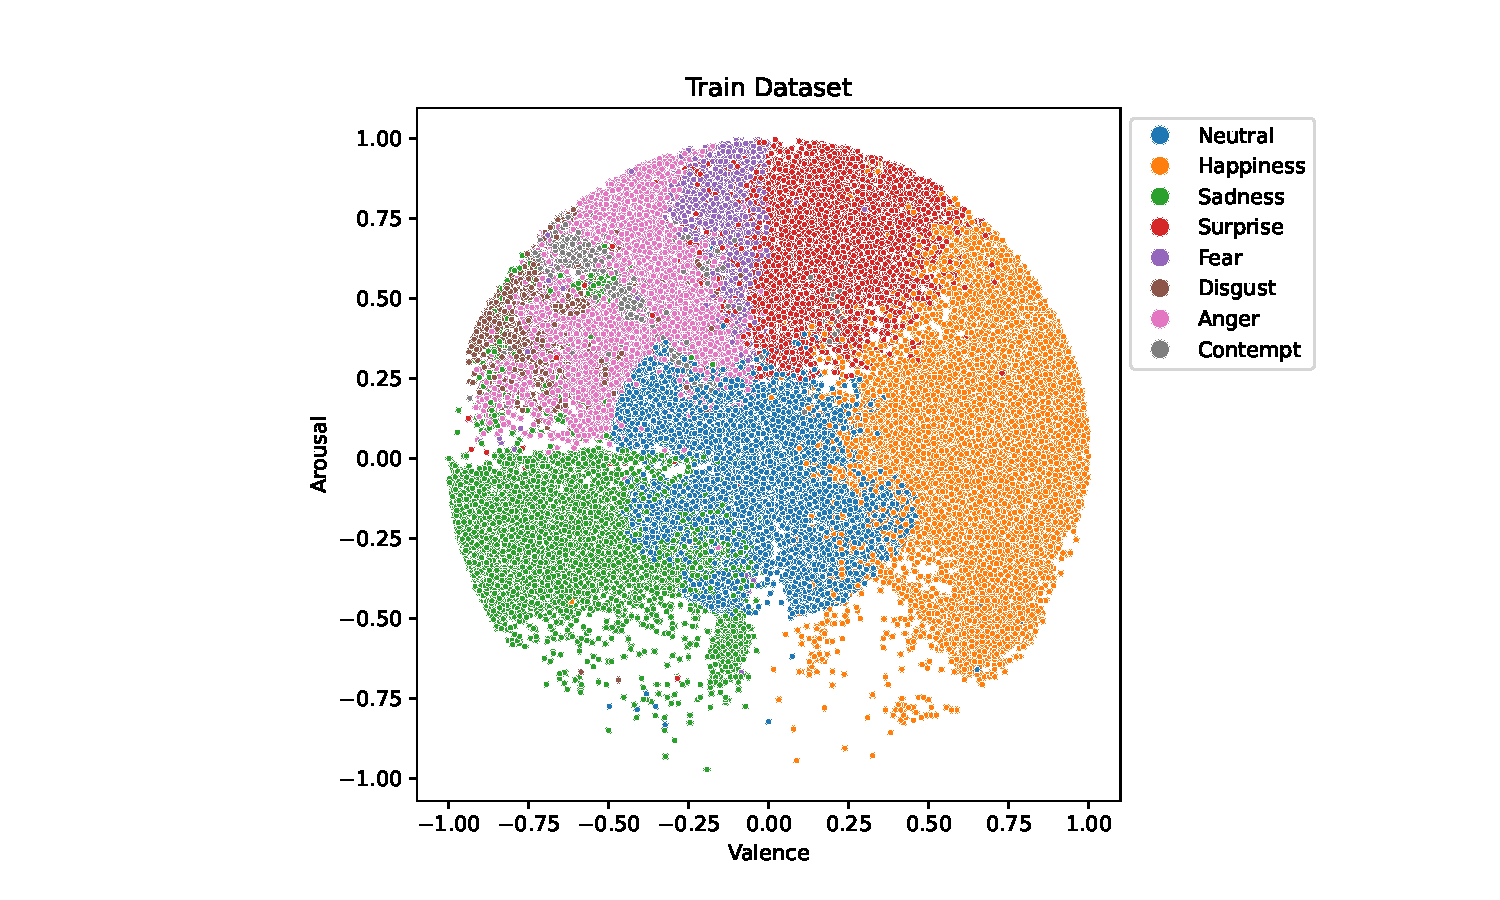
\includegraphics[width=\columnwidth, trim={4cm 0 2.5cm 0}, clip]{pictures/affectnet/scatterplot.pdf}
    \caption{\VA{} in a subset of the train dataset of \affectnet{} sorted by expression category.}
    \label{fig:scatterplot}
\end{figure}

\subsection{\affectnet{}}

Images in the \affectnet{}~\cite{mollahosseini2017affectnet} dataset are labeled with (1) one out of eight possible discrete expression categories, (2) a \val{} value as a real number between -1 and 1, (3) an \aro{} value as a real number between -1 and 1, and (4) facial landmark points. The distribution of discrete categories (see Figure~\ref{frequence\affectnet{}}) is unbalanced. %, leading to a weighted loss function for model training. 
The sum of the probabilities would lead up to 70\% only with two of the eight expression categories (\textit{happiness} and \textit{neutral}). On the other hand, validation data is evenly distributed across all labels.





To analyze the distribution of the continuous values \va{}, we displayed the values from the training set in the circumplex model of affect as originally proposed by Russell~\cite{rusellmodell}, with the values of \aro{} on the ordinate and \val{} on the abscissa (see Figure~\ref{fig:scatterplot}). As a result, the visualization clearly reveals that different expression categories can lead to an overlap in the \val{}/\aro{} values. Additionally, we analyze the distribution of \val{}/\aro{} per category as shown in  Figure~\ref{fig:affectnet_av_for_each_category}. For example, \textit{neutral} and \textit{happiness} expressions share a similar median in \aro{} dimension, whilst having a different median in the \val{} dimension. As expected, the \textit{neutral} category is centered around zero for \va{}. 

% \begin{figure}[ht]
%     \centering
%     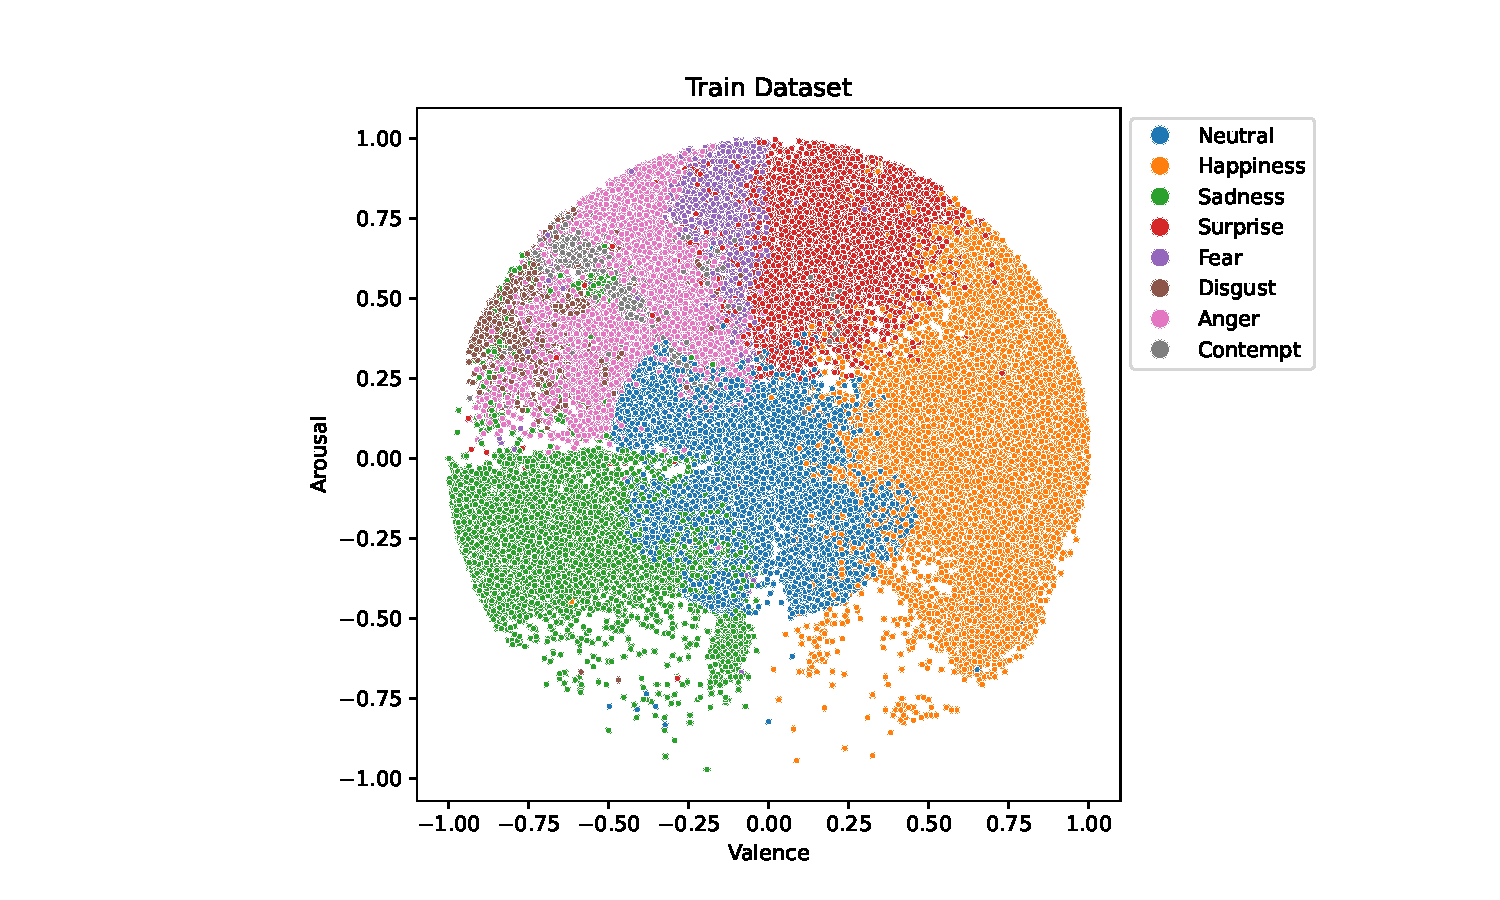
\includegraphics[width=\columnwidth]{pictures/affectnet/scatterplot.pdf}
%     \caption{Valence and Arousal sorted by Category}
%     \label{fig:scatterplot}
% \end{figure}

%\input{pictures/affectnet/frequency_of_expression.pgf}


\begin{figure}[t]
    \centering
    \includegraphics[width=0.65\columnwidth]{pictures/affectnet/av_for_each_category.pdf}
    \caption{\VA{} in \affectnet{}-8.}
    \label{fig:affectnet_av_for_each_category}
\end{figure}

A comparison of the \va{} values across the train and validation datasets shows that imbalance is also present.
\begin{figure}
    \centering
    \includegraphics[width=0.65\columnwidth]{pictures/affectnet/valence_distribution.pdf}
    \includegraphics[width=0.65\columnwidth]{pictures/affectnet/arousal_distribution.pdf}
    \caption{\Val{} and \Aro{} in \affectnet{}-8.}
    \label{fig:valence_distribution}
\end{figure}
In particular, more values from the training dataset are positive compared to the validation dataset with a higher portion of negative values (see Figure~\ref{fig:valence_distribution}). This imbalance is even more noticeable for arousal values. In the validation dataset, there are far more high-valued positive values compared to the training dataset.

\subsection{\emotic{}}
In \emotic{}~\cite{kosti_emotic_2017},  every image has a more complex labeling, targeting an overall context and a body focusing on the expression (see Figure~\ref{fig:example-imgs}). Each bounding box of a human is labeled with at least one expression, a \val{} value (integer between 1 and 10), an \aro{} value (integer between 1 and 10), a \dom{} value (integer between 1 and 10), gender (female/male) and age of a person (kid/teenager/adult).

% \begin{itemize}
%     \item Bounding box (Bbox) of the body image ([$x_1$ $y_1$ $x_2$ $y_2$])
%     \item Multi-labeling: At least one emotion
%     \item A \val{} value (integer between 1 and 10)
%     \item An \aro{} value (integer between 1 and 10)
%     \item A \dom{} value (integer between 1 and 10)
%     \item 
%     \item Age of the person in the Bbox (kid, teenager or adult)
% \end{itemize}

\newcolumntype{C}{>{\centering\arraybackslash}X} 

\begin{figure}[ht]
    \centering
    \includegraphics[width=\columnwidth]{pictures/emotic/frequency_of_expression.pdf}
    \caption{Distribution of expression frequency in \emotic{} train data.}
    \label{fig:emotic_labeldistr}
\end{figure}

Figure~\ref{fig:emotic_labeldistr} shows the relative occurrence of each expression in the dataset. Due to the multi-labeling of the dataset, an image can have multiple labels. Also, the overall frequency of the expression \textit{engagement} is dominating. %, leading to a weight in our loss function. 
Furthermore, all categories with a relative occurrence over 10\% are  "positive", corresponding to a positive \val{} value. 

Analysis of the label frequency in subsets has shown, that the training dataset contains a lot of images with one, two, or three categories, consistently decreasing. On the other side, the validation and the training dataset have a lot of images labeled with four or more categories  (see Figure~\ref{fig:emotic_label_occurance}). 

\begin{figure}[t]
    \centering
    \includegraphics[width=0.66\columnwidth]{pictures/emotic/frequency_of_expressions.pdf}
    \caption{Instances of multiple true expressions per image in \emotic{} data.}
    \label{fig:emotic_label_occurance}
\end{figure}

In summary, the \emotic{} dataset leads to a much more challenging task to train a suitable computer vision model. A fairly small dataset size, multi-person context, multi-label encoding, inconsistent unbalanced datasets, and different expression frequencies have led us to much more severe effort in the choice of suitable model hyperparameters.

